% ICRA draft. Swap to \documentclass[conference]{IEEEtran} once IEEEtran is
% installed (sudo tlmgr install ieeetran). The CUT below is the substantive
% work; the class swap is mechanical.
\documentclass[10pt,twocolumn,letterpaper]{article}
\usepackage[margin=0.75in]{geometry}
\setlength{\columnsep}{0.25in}
\usepackage{amsmath,amssymb}
\usepackage{booktabs}
\usepackage{graphicx}
\usepackage{microtype}
\usepackage[hidelinks]{hyperref}
\usepackage[numbers,sort&compress]{natbib}
\usepackage{caption}
\captionsetup{font=small}

\title{\bfseries Learning Location, Not Looking:\\
A Placement-Memorization Audit and Ten-Episode Repair at the 30M Scale}
\author{Anonymous submission}
\date{}

\begin{document}
\maketitle

\begin{abstract}
Fixed-placement benchmarks let imitation policies learn \emph{location} instead
of \emph{looking}. On LIBERO-Object we measure the preconditions exactly: the
target's start pose is bit-identical across all 50 shipped init states in 6 of
10 tasks, and the ten tasks between them use just \textbf{two} table positions,
22\,cm apart. A policy that memorizes two coordinates can present as
generalizing over ten.

We audit our own stack and find placement memorization at \textbf{four} layers:
a calibrated expert whose offset constant encodes pose, an iteration-coupled
selection loop, a grasp head whose regression prefers proprioception to pixels,
and a place head that memorized a command$\to$location map against a basket that
never moves. Three are repaired, each by \emph{data} rather than architecture:
ten placement-teleported episodes, command coverage in training, and DAgger on
the machine's own deployment viewpoints. The released head scores 0.700
held-out (35/50 $[0.56,0.81]$) and 0.520 randomized (26/50) where free per-tick
regression scores 0/56; a third object crosses at 18/50 $[0.24,0.50]$ against a
same-seed control at 3/50 (exact McNemar $p{=}6.1\times10^{-5}$). Twin control
cells scope that verification from both sides: the behavioural certificate is
joint in \emph{(head, stack)}---a detector-stack rebuild inverts which head
looks better.

The platform is 30.2\,M parameters deployed with \emph{no} language model---an
open-vocabulary detector's own text tower supplies every text embedding---which
makes it the smallest surveyed language-conditioned policy under both size
conventions at once. Nothing below is attributed to size.

Two annotation-free probes generalize past this artifact. Comparing two
instructions' detections on one frame exposes a grounding stage that
\emph{ignores} the instruction; swapping the instruction exposes one that
\emph{memorized} it. Applied here they show that object selection, approach and
grasping run with no language input at all: this system's entire language
channel is one latched place coordinate.

All results are simulation, one task and one object per claimed cell. Seven
pre-registered predictions were falsified and eight instruments retired at
their own calibration gates; two proposed mechanisms were tested and retracted
before reaching this paper.
\end{abstract}

\section{Introduction}

A policy that scores 0.700 on a manipulation benchmark has, on the face of it,
learned to see, decide, and act. This paper is about how much of such a number
can instead be \emph{location}: constants---in a benchmark's init files, in an
expert's calibration, in a learned regressor's shortcut---that encode where the
object always is, so that vision only ever gates an approach a memorized value
finishes. On LIBERO-Object~\citep{liu2023libero} we measure the preconditions
exactly: the target object's start pose is bit-identical across all 50 shipped
init states in 6 of 10 tasks, and varies by only 0.25--0.58\,cm (std) in the
other four. \emph{Across} tasks the structure is tighter still --- the ten
targets occupy just \textbf{two} table positions, 22.0\,cm apart, five tasks
each, agreeing to 0.0--0.7\,mm within a group. A policy that memorizes two
coordinates can present as generalizing over ten tasks. A benchmark with
${\lesssim}1$\,cm of within-task target variance and two positions between them
admits position-memorizers, and we found them in every layer of our own system.

The vehicle is MicroVLA, a deliberately small language-conditioned
vision-language-action stack: ${\sim}30$M parameters deployed, with a frozen
open-vocabulary detector serving as the only vision \emph{and} text encoder.
The size is the paper's setting, not its claim. Its methodological value is
that a stack this small has no capacity to paper over systems defects, so every
seam had to be instrumented---and the instruments are what this paper
contributes.

\paragraph{Contributions.}
\begin{enumerate}\itemsep2pt
\item \textbf{A placement-memorization audit and its verification method.}
A forensically worked instance of shortcut
learning~\citep{geirhos2020shortcut,dehaan2019causal} on a fixed-placement
benchmark, shown at four layers, with the corrected measured account of what
LIBERO-Object pins (per-task table and shipped measurement script); and the
probe-plus-behavioural-randomization protocol, motivated by the on-manifold
limit of substitution probes and by a counterexample to probe-only
certification. The protocol's twin control cells sharpen its scope:
behavioural randomization separates memorized from repaired heads under
identical draws on the deployment stack (1/10 vs.\ 4/10), and fails to
separate them on a stack whose rebuild disables visual goals (6/10 vs.\ 0/10).
\item \textbf{A controlled policy-class result.} With perception, trunk, and
corpus regime fixed, free per-tick regression scores 0/56 (upper 95\% bound
6.4\%) while goal-space supervision driving an engineered pick-and-place shell
scores 4/10 dev, 7/10 held-out, 4/10 randomized---claimed strictly as a bundle,
with the shell's share measured on both stacks.
\item \textbf{Training--serving-skew instrumentation.} 29 worked defect
instances at producer/consumer seams, split into disagreements catchable by
parity testing and agreements-on-a-wrong-convention catchable only by
provenance~\citep{sculley2015debt,breck2017mltest}.
\item \textbf{A ground-truth-free test for identity-blind grounding, and the
negative result it produced.} Open-vocabulary detectors are typically prompted
with a fallback chain, so a policy can appear language-conditioned while every
instruction collapses to the same generic prompt. Comparing two \emph{different}
instructions' selections on the same frame detects this without knowing which
is correct---the property that let it succeed where six ground-truth-seeking
instruments failed. Applied to our own stack it returns the same box for
different objects (median centre distance $0.0001$), so our best cell's 0.700 is
\emph{not} explained by binding the named object. Its behavioural companion is
equally cheap: \textbf{swap the instruction to a different object and rescore
against the original task}. Neither needs annotation, both need only a second
forward pass, and they fail differently---the first exposes a grounding stage
that ignores the instruction, the second a stage that memorized it. The swap is
what found our fourth memorization layer, and it works precisely where a fixed
benchmark cannot: when every task shares a target, a memorized
command$\to$location map and a grounded one are behaviourally identical until
the command is changed. Both ship as \texttt{eval/probes.py} with a test suite,
and their verdicts refuse the three over-claims this campaign got burned by:
too few co-detected frames returns \textsc{inconclusive} rather than a rate; a
discriminating result states that it cannot see whether the discrimination is
\emph{correct}; and an underpowered cell prints its own ceiling.
\end{enumerate}

\noindent Both headline findings have one shape: apparent competence resting on
a channel other than the claimed one---position where we claimed looking, shape
where we claimed naming. The audit generalizes better than the artifact does.

\section{Platform}

\begin{table}[h]\centering\small
\caption{Deployed parameter ledger. ``Deployed'' counts every parameter loaded
at inference, frozen or trained.}
\begin{tabular}{lrl}
\toprule
component & params & status \\
\midrule
YOLO-World-S detector (vision \emph{and} the only text encoder) & 13.0\,M & frozen \\
Tiny Recursive Model world model & 9.97\,M & frozen at deployment \\
fusion + drift + relational + planner trunk heads & 7.0\,M & trained ($\le$9\,M cap) \\
goal heads (grasp 0.17\,M + place 0.07\,M) + learned gates & 0.24\,M & trained \\
\midrule
\textbf{deployed total} & \textbf{30.2\,M} & \\
\bottomrule
\end{tabular}
\end{table}

No separate language model exists anywhere in the stack: the command is parsed
into source/target phrases, and CLIP embeddings for (command, source, target)
are harvested once per task from the detector's own text tower. \textbf{The
world model is causally inert in every nonzero number of this paper}---a
persistence-TRM ablation reproduces the held-out cell exactly (0.700).

\section{Results}

\begin{figure}[t]\centering

\includegraphics[width=\textwidth]{../visuals/F3_protocol_by_head.png}
\caption{Protocol $\times$ head, Wilson 95\% intervals. The memorized head leads
on \emph{dev} and collapses on held-out and randomized; the released head is
flat across all three. The randomized panel's inset is the audit-stack control,
where the separation \emph{inverts} (memorized 6/10, released 0/10) --- it is
never pooled with the deployment-stack bars, which is why the behavioural
certificate is joint in (head, stack). Free per-tick regression, same trunk and
corpus regime, scores 0/56.}
\label{fig:protocol}
\end{figure}

\begin{table}[h]\centering\small
\caption{Protocol $\times$ head. All cells $k/10$ with Wilson 95\% intervals;
task 0, wrist camera. Audit-stack cells are never pooled with deployment-stack
cells (\S\,stack finding).}
\begin{tabular}{lcccc}
\toprule
protocol & memorized head & \textbf{flagship (released)} & sibling A & sibling B \\
\midrule
dev (states 0--9)            & 7/10 & 4/10 & 7/10 & 7/10 \\
held-out (states 10--19)     & 3/10 & \textbf{7/10} & 7/10 & 6/10 \\
randomized $\pm4$\,cm (same draws) & \textbf{1/10} & \textbf{4/10} & 5/10 & 3/10 \\
randomized $\pm4$\,cm (audit stack) & 6/10 & 0/10 & --- & --- \\
\bottomrule
\end{tabular}
\end{table}

\noindent Confirmed at power: held-out \textbf{35/50 $=0.700$
$[0.56,0.81]$}; randomized \textbf{26/50 $=0.520$ $[0.39,0.65]$}.
Across a detector-stack rebuild the repaired head reproduces in all three
protocols while the memorized head's dev cell collapses $7/10\to2/10$ to its
held-out floor: memorization is stack-coupled, \emph{visual} grounding---which
input the head reads---is what survived.

\begin{figure*}[t]\centering
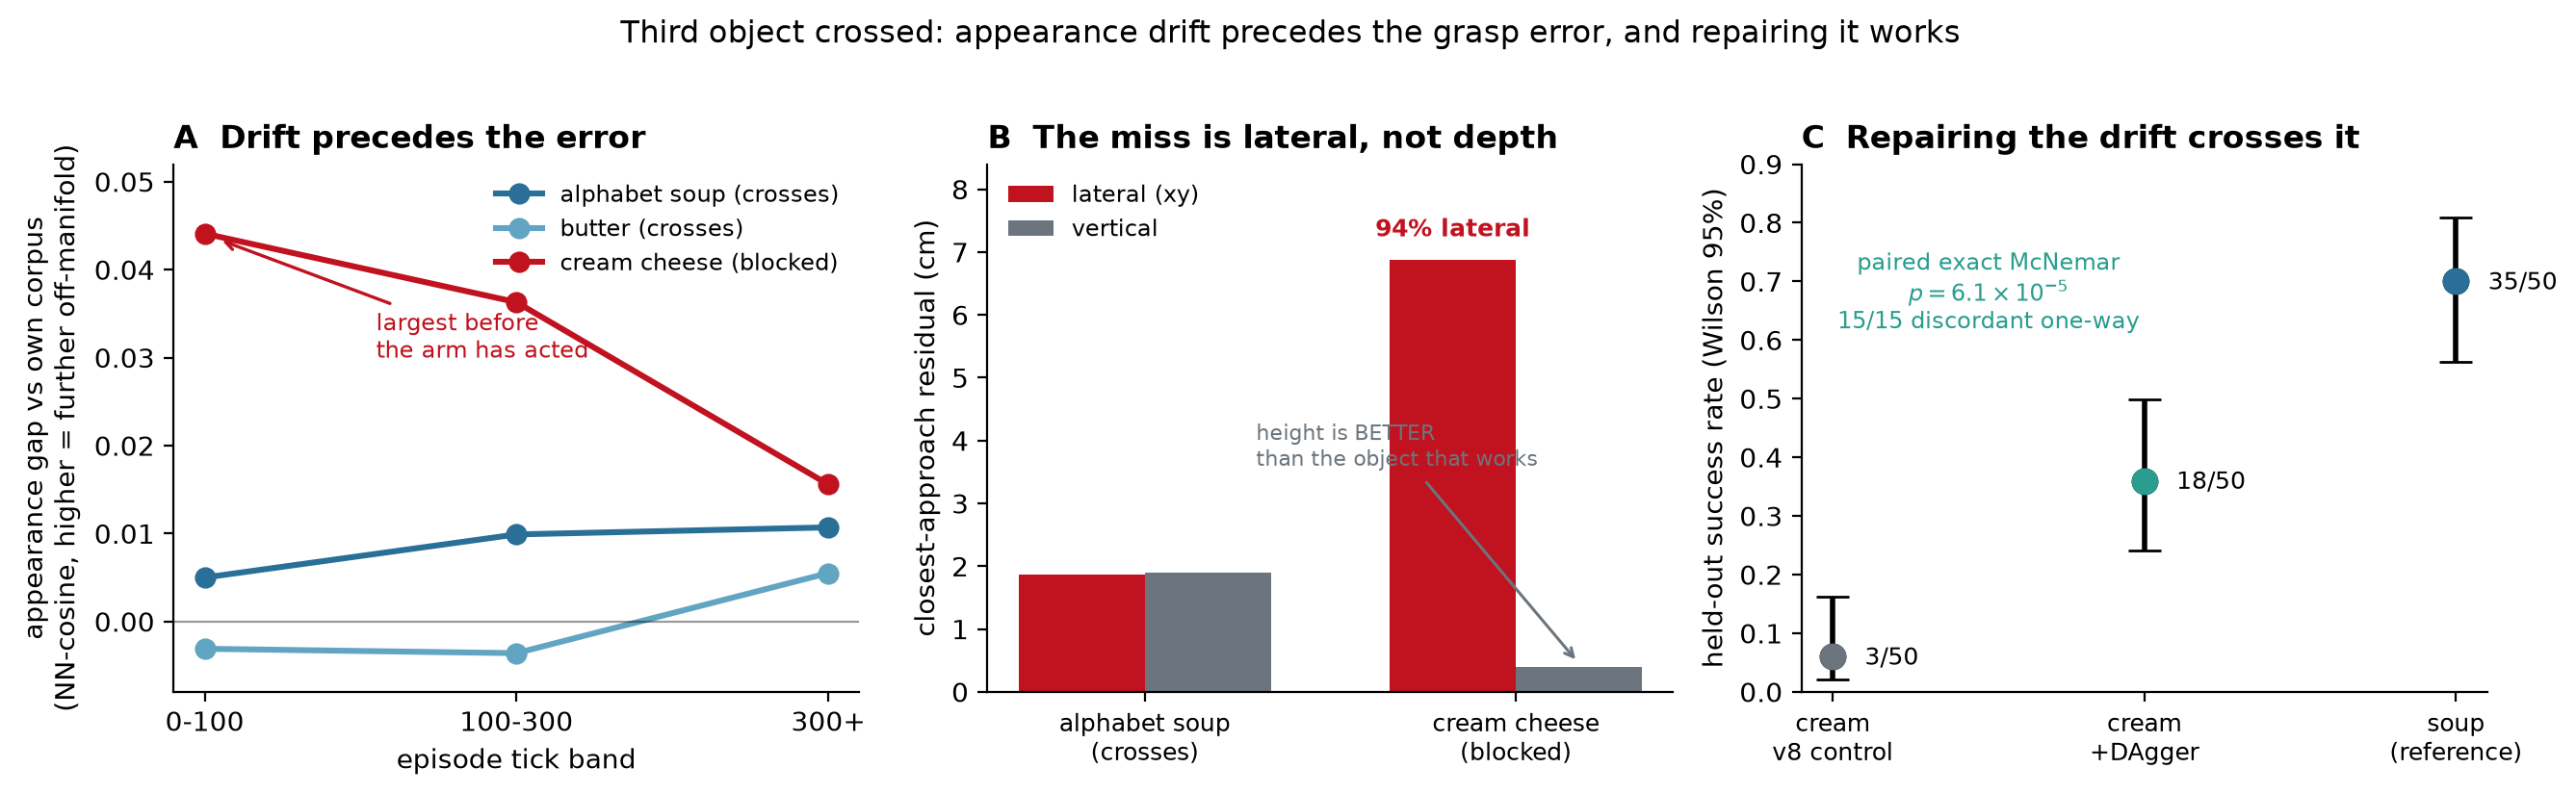
\includegraphics[width=0.92\textwidth]{../visuals/F5_third_object.png}
\caption{How the third object crossed. \textbf{(A)} The blocked object's
appearance drift is largest \emph{before the arm has acted} and shrinks 65\%,
where both crossing objects show the opposite rising trend --- the circularity
check that retired two earlier instruments. \textbf{(B)} The miss is 94\%
lateral, with the blocked object's \emph{height} better than the crossing
object's. \textbf{(C)} The intervention, $n{=}50$ per arm on identical seeds:
3/50 $\to$ 18/50 (paired exact McNemar $p{=}6.1\times10^{-5}$), against the
crossing object's 35/50.}
\label{fig:third}
\end{figure*}

\section{Multi-object addendum}

Four objects were attempted and three cross: 35/50, a second confirmed twice on
never-scored seeds, and a third at \textbf{18/50 $[0.24,0.50]$} against a
same-seed control at 3/50 (paired exact McNemar $p{=}6.1\times10^{-5}$). The
fourth's scripted teacher never reached a grasp, so no corpus exists for it; it
is untested rather than failed.

For the third object we proposed nine mechanisms and \textbf{refuted eight by
measurement}: generic-tail indiscriminability, box-centre spread, proposal
scarcity, misbinding, position memorization, descent failure, binder quality,
and uv-tail extrapolation. Two were our own and were retracted before reaching
this paper. The object is notably \emph{not} misbinding: a world-space probe
finds it reaches the commanded object 6/6, failing by a systematic 6.9\,cm
\emph{lateral} error (coherence 0.976) with height \emph{better} than the
object that works.

The surviving mechanism is appearance-side off-manifold drift, and it survives
three tests. \emph{Falsification}: the blocked object's deployment embeddings
sit $3.1\times$ further from its own corpus than the crossing object's, and the
second crossing object---predicted before it ran---has the smallest gap of all.
\emph{Circularity}: a wrong goal would itself produce unusual viewpoints, so we
split by tick; drift is largest in the first 100, before the arm has acted, and
shrinks 65\%, while the crossing objects show the opposite rising trend.
\emph{Intervention}: fine-tuning the grasp head on the machine's own viewpoints
---labelled from the simulator's object pose, which the corpus cannot supply
for viewpoints the teacher never visited---cuts the deployed lateral error
56\% ($p{=}0.020$) and produces the cell above. Collection drew seed 0 and
evaluation seed 20, so no cell is scored on its own band.

The repair is \textbf{specific}, which is its best evidence. Applied to the
object that already works it changes nothing: 28/50 vs.\ a 27/50 control, 21
discordant pairs split 11--10, $p{=}1.0000$. Three times the drift, six times
the benefit; a third of the drift, none at all. A repair improving every object
would be consistent with generic regularization; one appearing only where the
measured defect is present is difficult to attribute otherwise. It repairs
\emph{covariate shift}, not absent labels, and only where viewpoints have
actually drifted.

\section{Related work}

Size is comparable only under a stated convention, and the two in common use
disagree about which system is smallest, because published counts routinely
exclude a frozen language encoder that inference nonetheless loads. We report
both (Table~\ref{tab:size}). Under \emph{trained parameters} the smallest
published alternative is Octo-small's 27\,M transformer~\citep{octo2024}, and
MicroVLA's 17.2\,M is $1.6\times$ below it; under \emph{deployed} $=$ every
parameter loaded at inference it is RT-1's 35\,M~\citep{brohan2022rt1}, and
MicroVLA's 30.2\,M is below that \emph{even after granting RT-1 a free language
encoder}---RT-1's count excludes the Universal Sentence Encoder producing its
instruction embedding, for which we cite no figure rather than estimate one.
MicroVLA is thus smallest under both conventions simultaneously, the strongest
form of the claim the evidence supports. The survey was run adversarially,
against systems whose stated goal is minimal size: NanoVLA-S is 52\,M trainable
atop a frozen ResNet18 \emph{and} a frozen BERT-base
(${\sim}161$\,M loaded)~\citep{nanovla2025}, and LiteVLA reaches a Raspberry Pi
on a 256\,M SmolVLM backbone~\citep{litevla2025}. Both sit above MicroVLA on
both axes, and NanoVLA is the convention gap in miniature---a paper named for
being nano, reporting 52\,M while loading ${\sim}161$\,M, because the frozen
language encoder is not counted.

\begin{table}[h]\centering\small
\caption{Size under both conventions. $\dagger$ excludes a frozen language
encoder the published count omits. Sizes only: capability, task breadth, and
protocol are not comparable.}
\label{tab:size}
\begin{tabular}{lrrl}
\toprule
system & trained & deployed & language encoder \\
\midrule
RT-2~\citep{brohan2023rt2}        & 55\,B & 55\,B & internal (PaLI-X) \\
OpenVLA~\citep{kim2024openvla}    & 7\,B  & 7\,B  & internal (Llama-2) \\
SmolVLA~\citep{shukor2025smolvla} & 450\,M & 450\,M & internal (SmolVLM2) \\
LiteVLA~\citep{litevla2025}       & LoRA only & ${\sim}256$\,M & internal (SmolVLM-256M) \\
NanoVLA-S~\citep{nanovla2025}     & 52\,M & 161\,M & BERT-base, frozen \\
Octo-small~\citep{octo2024}       & \underline{27\,M} & 138\,M & T5-base, 111\,M frozen \\
RT-1~\citep{brohan2022rt1}        & 35\,M & \underline{$\ge$35\,M}$^\dagger$ & USE, frozen, uncounted \\
\midrule
\textbf{MicroVLA}                 & \textbf{17.2\,M} & \textbf{30.2\,M} & \emph{none}---detector's own tower \\
\bottomrule
\end{tabular}
\end{table}

The claim is bounded and checkable: it ranges over language-conditioned VLA
policies with published parameter counts that we surveyed, it is a statement
about parameter counts alone, and it is refuted by exhibiting any surveyed-class
system below 17.2\,M trained or 30.2\,M deployed. We cannot rule out
unpublished or unsurveyed smaller systems. ``Language-conditioned'' here names
the \emph{reference class} --- systems that accept a language instruction ---
and is not a claim about how much work that instruction does in ours: the
decomposition above shows it reduces to one latched place coordinate. A reader
who thinks that disqualifies the artifact from the class should read the size
row as smaller still, not larger. The mechanism behind the gap is
architectural rather than incidental: MicroVLA carries no separate language
model at all, because the detector's own text tower supplies every text
embedding---so the frozen encoder that the other rows pay for twice (once in
memory, once in the convention mismatch) does not exist here. Of MicroVLA's
17.2\,M trained parameters only 7.24\,M are causally load-bearing, since the
9.97\,M world model is inert in every nonzero number of this paper.
No number here is comparable to
community-protocol LIBERO scores (600 steps, $n{=}10$, wrist-only,
scripted-expert corpora). Predicting \emph{where} rather than \emph{how} is
the Transporter~\citep{zeng2020transporter} and CLIPort~\citep{shridhar2021cliport}
lineage, continued by keypoint interfaces over engineered
primitives~\citep{liu2024moka,huang2023voxposer} and, with both levels
learned, $\pi_{0.5}$~\citep{black2025pi05}. Our audit is a worked manipulation
instance of causal confusion and copycat
shortcuts~\citep{dehaan2019causal,wen2020copycat,bansal2018chauffeurnet};
what we add is the audited counterexample to probe-only certification, the
resulting probe-plus-randomization pairing, and the control cells that scope
the pairing itself. Bootstrapping from scripted experts is
established~\citep{mandlekar2023mimicgen}; our delta is that the scripted
teacher is itself audited, caught encoding placement and detector version, and
repaired.

\section{Claims, non-claims, limitations}

\textbf{Claimed:} the pinning measurement in its scoped form; the released
head's cells above; free per-tick regression at 0/56; the de-memorization
mechanism at the head level (attribution shift, varied-label validation, and a
paired jitter ablation, $0/10\to7/10$ dev, exact McNemar/sign $p\approx0.016$),
scoped by the audit-stack control; 29 worked skew defects; the bounded size
result of Table~\ref{tab:size} (smallest of the surveyed systems under both the
trained and the deployed convention simultaneously); and the identity-blindness
of deployed role binding, together with its architectural corollary that no
text embedding reaches the grasp head---claimed as a property \emph{of this
system}, and offered as a test other detector-grounded policies can run, not as
a claim about them.
\textbf{Not claimed:} any task-success contribution from the world model
(causally inert in every nonzero number); end-to-end learned motor control (the
shell is engineered); head-level grounding from the randomized column alone,
stack-free; object-level generalization beyond the addendum's two crossed
objects (four attempted, three crossed; the fourth's scripted teacher never
reached a grasp, so no corpus exists for it and it is untested rather than
failed); any
deployed binding-accuracy figure beyond the world-space nearest-body counts;
physical deployment; any size claim beyond
Table~\ref{tab:size}'s bounded one (surveyed systems, published counts,
parameters only)---neither that smaller systems cannot exist, nor that small
size caused any result here.
\textbf{Limitations:} $n{=}10$ per cell with $n{=}50$ confirmations on two
protocols; ten held-out states reused across five disclosed selection looks;
machine constants inherited from a dev-tuned era; substitution probes are
on-manifold; $\pm4$\,cm randomization sits inside the shell's $\pm6$\,cm probe
envelope and separates heads only where visual goals are live; the teacher's
calibration consumed privileged telemetry offline; single benchmark, single
simulator.

\bibliographystyle{plainnat}
\bibliography{refs}

\end{document}
